\documentclass[11pt,a4paper]{article}

% ---------------------------------------------------------------------------
% Thermodynamic compatibility of interacting autocatalytic cores:
% an exact phase diagram and a layered obstruction theory.
%
% Author metadata: set the three macros below before submission.
% ---------------------------------------------------------------------------
\newcommand{\PaperAuthor}{Anonymous manuscript}
\newcommand{\PaperAffiliation}{}
\newcommand{\PaperDate}{September 7, 2026}

\usepackage[T1]{fontenc}
\usepackage[utf8]{inputenc}
\usepackage{lmodern}
\usepackage{microtype}
\usepackage[a4paper,margin=1.05in]{geometry}
\usepackage{amsmath,amssymb,amsthm,mathtools}
\usepackage{booktabs}
\usepackage{array}
\usepackage{enumitem}
\usepackage{xcolor}
\usepackage{graphicx}
\usepackage{tikz}
\usetikzlibrary{arrows.meta,positioning,calc}
\usepackage{listings}
\usepackage{url}
\usepackage[numbers,sort&compress]{natbib}
\usepackage[colorlinks=true,linkcolor=blue!55!black,citecolor=blue!55!black,urlcolor=blue!55!black]{hyperref}

\setlist{itemsep=2pt,topsep=3pt}
\setlength{\emergencystretch}{1.5em}

\theoremstyle{plain}
\newtheorem{theorem}{Theorem}[section]
\newtheorem{proposition}[theorem]{Proposition}
\newtheorem{lemma}[theorem]{Lemma}
\newtheorem{corollary}[theorem]{Corollary}
\theoremstyle{definition}
\newtheorem{definition}[theorem]{Definition}
\newtheorem{example}[theorem]{Example}
\newtheorem{hypothesis}[theorem]{Hypothesis}
\theoremstyle{remark}
\newtheorem{remark}[theorem]{Remark}
\newtheorem{question}[theorem]{Question}

\lstdefinelanguage{Lean}{
  morekeywords={theorem,def,structure,inductive,namespace,end,import,by,intro,exact,constructor,refine,where,abbrev,noncomputable,rintro,simpa,using},
  sensitive=true,
  morecomment=[l]{--},
  morestring=[b]",
}
\lstset{
  language=Lean,
  basicstyle=\ttfamily\small,
  keywordstyle=\bfseries,
  commentstyle=\itshape\color{black!60},
  columns=fullflexible,
  keepspaces=true,
  breaklines=true,
  frame=single,
  framerule=0.3pt,
  xleftmargin=1em,
  xrightmargin=1em,
  extendedchars=true,
  literate={≤}{{$\le$}}1 {≥}{{$\ge$}}1 {ℕ}{{$\mathbb{N}$}}1 {ℝ}{{$\mathbb{R}$}}1 {→}{{$\to$}}1 {∀}{{$\forall$}}1 {∃}{{$\exists$}}1 {≠}{{$\neq$}}1 {∧}{{$\wedge$}}1 {¬}{{$\neg$}}1 {↔}{{$\leftrightarrow$}}1 {∑}{{$\sum$}}1 {∏}{{$\prod$}}1 {₀}{{$_0$}}1 {₁}{{$_1$}}1 {₂}{{$_2$}}1 {⟨}{{$\langle$}}1 {⟩}{{$\rangle$}}1 {∈}{{$\in$}}1 {·}{{$\cdot$}}1 {α}{{$\alpha$}}1 {β}{{$\beta$}}1 {μ}{{$\mu$}}1
}

\newcommand{\R}{\mathbb{R}}
\newcommand{\N}{\mathbb{N}}
\newcommand{\Z}{\mathbb{Z}}
\newcommand{\Rpos}{\R_{>0}}
\newcommand{\cS}{\mathcal{S}}
\newcommand{\cR}{\mathcal{R}}
\newcommand{\cC}{\mathcal{C}}
\newcommand{\cK}{\mathcal{K}}
\newcommand{\cF}{\mathcal{F}}
\newcommand{\MPAC}{\mathsf{MultiPAC}}
\newcommand{\MCAC}{\mathsf{MultiCAC}}
\newcommand{\DIR}{\mathsf{Dir}}
\newcommand{\LIN}{\mathsf{LinCx}}
\newcommand{\lean}[1]{\texttt{#1}}
\newcommand{\rev}{\rightleftharpoons}
\DeclareMathOperator{\supp}{supp}

\title{Thermodynamic compatibility of interacting autocatalytic cores:\\ an exact phase diagram and a layered obstruction theory}
\author{\PaperAuthor\\ \PaperAffiliation}
\date{\PaperDate}

\begin{document}
\maketitle

\begin{abstract}
A potential autocatalytic core (PAC) is a minimal stoichiometric motif that admits a strictly productive reaction current; a consistent autocatalytic core (CAC) is a PAC whose productive current is realized by a positive concentration vector under thermodynamically consistent mass-action kinetics. Kosc, Kuperberg, Rajon and Charlat (\emph{Proc.\ Natl.\ Acad.\ Sci.\ USA}, 2025) proved that every isolated PAC is a CAC, and exhibited two overlapping cores that admit a common productive current but no common concentration vector. We study when a family of interacting cores admits one common thermodynamic realization, with all cores sharing a single activity vector and fixed transition-state factors. First, we refute the natural strengthening of the isolated-core theorem: there is a two-core family with a common productive current and a common strict reaction-direction potential that nevertheless has no common realization. The obstruction is metric rather than directional: it already defeats the linear relaxation in which every distinct stoichiometric complex receives an independent activity. Second, for the responsible topology, two autocatalytic triangles $A\rev B\rev C\rev 2A$ and $A\rev B\rev D\rev 2A$ sharing $A\rev B$, we prove an exact phase diagram: with private transition-state factors in ratio $k$, a common realization exists if and only if $1/2<k<2$, and for arbitrary positive factors if and only if the reciprocal-factor sums of the two private branches are within a factor of two. In transition-state language the symmetric window is $|\Delta G^{\ddagger}|<RT\ln 2$. Third, we derive an interface calculus: eliminating a gain-$m$ triangle with factors $b_0,b_1,b_2$ leaves exactly the open response interval $(R/m,R)$ with $R=b_0(1/b_1+1/b_2)$, and two eliminated cores compose precisely when their intervals overlap. Fourth, we show that the linear relaxation is not the whole story: a two-species, three-reaction family passes the flow, direction and independent-complex tests but fails the monomial lift to a common species-activity vector. Together with the direction obstruction of the original example, this yields three provably distinct failure mechanisms. All headline theorems are formalized in Lean~4 against Mathlib with warnings promoted to errors and no admitted statements.
\end{abstract}

\noindent\textbf{Keywords.} autocatalysis; autocatalytic cores; chemical reaction networks; mass-action kinetics; thermodynamic consistency; transition-state theory; phase diagram; toric geometry; formal verification.

\medskip
\noindent\textbf{MSC 2020.} 92E20, 80A30, 90C05, 14M25, 68V20.

\section{Introduction}\label{sec:intro}

Autocatalysis, the ability of a set of chemical species to catalyse its own net production, is widely regarded as a prerequisite for the emergence of Darwinian dynamics in chemistry \citep{blokhuis2020,hordijk2004,steel2020}. Blokhuis, Lacoste and Nghe \citep{blokhuis2020} identified autocatalysis with a stoichiometric property of a reaction network: a motif is autocatalytic when some reaction current strictly increases the concentration of each of its species, and they classified the minimal such motifs, the \emph{autocatalytic cores}, into five topological types. Cores are purely combinatorial objects. They know nothing about rate constants, concentrations or free energies, and the question of whether a stoichiometrically autocatalytic motif can actually run under thermodynamically consistent kinetics was left open by that classification.

Kosc, Kuperberg, Rajon and Charlat \citep{kosc2025} addressed this question. They defined a \emph{potential autocatalytic core} (PAC) as a minimal autocatalytic motif of a reaction network and a \emph{consistent autocatalytic core} (CAC) as a PAC whose productive current is the current induced, under mass-action kinetics constrained by local detailed balance, by some positive concentration vector. They proved that PAC detection is NP-complete, and, more importantly for the present paper, that \emph{every PAC is a CAC}: for any activation barriers and any standard free energies, an isolated PAC can always be made to run in the productive direction if concentrations are unbounded. They also observed that this realizability does not survive interaction. Their Figure~4 exhibits two PACs which share reactions, which admit a common productive current (a \emph{multiPAC}), and which cannot be simultaneously consistent: no single concentration vector makes both cores productive, whatever the barriers.

This paper is about the structure hidden in that observation. When several cores share species and reactions, a common realization has to satisfy simultaneously the polyhedral productivity constraints of each core, the sign constraints on each reaction direction, the magnitude constraints imposed by fixed transition-state factors, and the algebraic constraints that tie the activity of each stoichiometric complex to a monomial in the species activities. It is natural to ask whether the polyhedral and sign constraints already decide the matter, as they do for one core. We call this the Strong Compatibility Hypothesis: \emph{if a family of cores admits a common productive current and a common strict direction potential, then it admits a common thermodynamic realization.} Our first result is that this hypothesis is false, and the way it fails organizes the rest of the paper.

\subsection{Main results}\label{sec:mainresults}

We work with a finite reversible reaction network $Q$ in which reaction $r$ has reactant complex $\alpha_r$, product complex $\beta_r$ and a positive \emph{transition-state factor} $b_r$; for a positive activity vector $z$ the oriented current is $j_r(z)=b_r(z^{\alpha_r}-z^{\beta_r})$. This is the Kosc et al.\ model with $b_r=e^{-G_r^{\ddagger}/RT}$ and $z_s=e^{\mu_s/RT}$ (Section~\ref{sec:setting}). A \emph{core family} is a finite collection of PACs of $Q$ together with a global orientation of every reaction. Four predicates on a core family are studied:
\begin{itemize}
\item $\MPAC$: some current $v$ has the prescribed sign on every reaction and makes every core productive;
\item $\DIR$ (direction compatibility): some potential $\mu\in\R^{\cS}$ has strictly positive oriented affinity $\varepsilon_r\langle\alpha_r-\beta_r,\mu\rangle$ on every reaction;
\item $\LIN$ (linear-complex compatibility): some assignment of an independent positive activity $y_c$ to every distinct complex $c$ makes the currents $b_r(y_{\alpha_r}-y_{\beta_r})$ correctly signed and every core productive;
\item $\MCAC$: some positive species vector $z$ makes the currents $j_r(z)$ correctly signed and every core productive.
\end{itemize}
$\MCAC$ implies each of the other three (Lemma~\ref{lem:necessary}); the three are otherwise independent filters on different projections of the problem. Our results are as follows; each is stated informally here and precisely in the body of the paper.

\begin{enumerate}[label=(\Alph*)]
\item\label{res:A} \textbf{Strong Compatibility fails (Theorem~\ref{thm:sch}).} The two autocatalytic triangles $A\rev B\rev C\rev 2A$ and $A\rev B\rev D\rev 2A$ sharing $A\rev B$, with factors $(1,1,1,10,10)$, form a family that is $\MPAC$ and $\DIR$ but not $\MCAC$. The obstruction already defeats $\LIN$: it is a conflict between fixed factor magnitudes, not between reaction directions. The original example of Kosc et al.\ fails for a different reason: it is not $\DIR$, a signed circuit of the six reactions forbids the required orientation (Proposition~\ref{prop:paperpair}).
\item\label{res:B} \textbf{Exact phase diagram (Theorem~\ref{thm:phase}).} For the same two triangles with private factors $(1,1)$ on the left and $(k,k)$ on the right, both cores are PACs and the family is $\MPAC$ and $\DIR$ for every $k>0$, while it is $\MCAC$ exactly when $1/2<k<2$. The endpoints are excluded because a strict productivity residual degenerates there. With arbitrary factors $b_0;b_1,b_2;b_3,b_4$ the condition becomes $\tfrac12<(1/b_3+1/b_4)/(1/b_1+1/b_2)<2$ (Proposition~\ref{prop:generalphase}).
\item\label{res:C} \textbf{Interface calculus (Theorem~\ref{thm:interface}, Corollary~\ref{cor:compose}).} Eliminating a gain-$m$ triangle $A\to B\to C\to mA$ with factors $b_0,b_1,b_2$ from the literal productive-current equations leaves the exact open interval $(R/m,R)$, $R=b_0(1/b_1+1/b_2)$, of admissible values for the ratio $q$ of the private complex-activity drop to the shared drop. Two such intervals with gains $m_L,m_R$ and coefficients $R_L,R_R$ intersect exactly when $1/m_L<R_R/R_L<m_R$. The phase diagram of~\ref{res:B} is the case $m_L=m_R=2$.
\item\label{res:D} \textbf{Monomial-lift obstruction (Theorem~\ref{thm:toric}).} The family $\{A\rev B,\ B\rev 2A\}$, $\{A\rev B,\ B\rev 3A\}$ with factors $(1,1,2)$ on two species and three reactions is $\MPAC$, $\DIR$ and $\LIN$ but not $\MCAC$. At the linear-complex level the two private response intervals are independent; the monomial lift couples them through the common activity of $A$ and empties their intersection.
\item\label{res:E} \textbf{Formal verification (Section~\ref{sec:formal}).} The statements in~\ref{res:A}--\ref{res:D}, including PAC minimality of every core involved, have been compiled in Lean~4 \citep{demoura2021} against Mathlib \citep{mathlib2020} with warnings treated as errors and no unproved declarations. The few hand-proved extensions are listed explicitly in Section~\ref{sec:notformal}.
\end{enumerate}

The picture that emerges is a layered one (Figure~\ref{fig:layers}). A common realization can fail at the level of reaction directions (a signed circuit), at the level of fixed magnitudes (a linear-complex wall) or at the level of the monomial lift (a toric-image wall), and the three examples of this paper show that each layer can fail while the previous ones hold. For the smallest interacting topology, two triangles with one shared edge, the complete answer is a single scalar interval, and its endpoints have a direct physical reading: in the symmetric family the two private branches must have Gibbs activation energies within $RT\ln 2$, about $1.7\,\mathrm{kJ\,mol^{-1}}$ at $298\,\mathrm{K}$, of each other (Section~\ref{sec:physics}).

\subsection{Relation to previous work}

The framework of autocatalytic cores is due to Blokhuis, Lacoste and Nghe \citep{blokhuis2020}; its diluted-regime dynamics were developed by Unterberger and Nghe \citep{unterberger2022} and Nandan, Nghe and Unterberger \citep{nandan2025}, and cores with explicit catalysis are treated by Golnik, Gatter, Stadler and Vassena \citep{golnik2026cores}. The polyhedral geometry of minimal autocatalytic subnetworks is studied by Gagrani, Blanco, Smith and Baum \citep{gagrani2024}; the NP-completeness of recognizing autocatalysis goes back to Andersen, Flamm, Merkle and Stadler \citep{andersen2012} and, for PAC detection, to Kosc et al.\ \citep{kosc2025}. Vassena and Stadler \citep{vassena2024} identify unstable cores as the source of dynamical instability; that question is orthogonal to ours, which concerns existence of a positive static witness. The relationship between cores and the RAF sets of Hordijk and Steel \citep{hordijk2004,steel2020} is clarified in \citep{golnik2026bridging}. Despons, De Decker and Lacoste \citep{despons2024} derive stoichiometric bounds on affinities at optimal flux; their regime, a steady state at maximal production, differs from the existence question treated here. The word ``toric'' is used below only for the monomial image of the species activities; it does not refer to the toric dynamical systems of Craciun, Dickenstein, Shiu and Sturmfels \citep{craciun2009}, which concern complex-balanced steady states in the sense of Feinberg \citep{feinberg2019}.

To our knowledge the exact factor-of-two window, the source-level interface interval and the separation of the three obstruction layers are new. This assessment is based on a bounded primary-source search completed on 31 August 2026 and is not a proof of absence.

\subsection{Organization}

Section~\ref{sec:setting} fixes the model and the four compatibility predicates. Section~\ref{sec:sch} refutes the Strong Compatibility Hypothesis. Section~\ref{sec:phase} proves the phase diagram, Section~\ref{sec:interface} the interface calculus and Section~\ref{sec:toric} the monomial-lift obstruction. Section~\ref{sec:formal} documents the formal verification and Section~\ref{sec:discussion} discusses the physical reading, limitations and open problems.

\section{Setting}\label{sec:setting}

\subsection{Reversible networks and barrier-weighted currents}

Let $\cS$ and $\cR$ be finite sets of species and reactions. A \emph{complex} is a vector $c\in\N^{\cS}$; for $z\in\Rpos^{\cS}$ write $z^{c}=\prod_{s}z_s^{c_s}$.

\begin{definition}[Reversible network]\label{def:crn}
A reversible reaction network is $Q=(\cS,\cR,\alpha,\beta,b)$ where $\alpha_r,\beta_r\in\N^{\cS}$ are the reactant and product complexes of $r\in\cR$ and $b_r>0$ is its transition-state factor. Its stoichiometric matrix is $N_{sr}=\beta_r(s)-\alpha_r(s)$. For $z\in\Rpos^{\cS}$ the \emph{current} of $r$ is
\begin{equation}\label{eq:current}
  j_r(z)=b_r\bigl(z^{\alpha_r}-z^{\beta_r}\bigr).
\end{equation}
\end{definition}

Equation~\eqref{eq:current} is the mass-action current of Kosc et al.\ \citep[Eq.~5]{kosc2025} in the ideal-solution regime with $RT=1$: if $\mu_s$ is the chemical potential of species $s$ and $G_r^{\ddagger}$ the Gibbs activation energy of reaction $r$, local detailed balance gives $v_r=e^{-G_r^{\ddagger}}\bigl(e^{\langle\alpha_r,\mu\rangle}-e^{\langle\beta_r,\mu\rangle}\bigr)$, which is~\eqref{eq:current} with $z_s=e^{\mu_s}$ and $b_r=e^{-G_r^{\ddagger}}$. The factor $b_r$ is a kinetic prefactor: it scales both directions of $r$ equally and does not affect the equilibrium constant. Throughout, $b_r$ is fixed and the free variable is $z$. Because $\mu_s$ absorbs the standard free energy of $s$, the results below hold for all standard free energies; the only thermodynamic input is the set of factors $b_r$.

\subsection{Motifs and potential autocatalytic cores}

The following definitions transcribe Definitions~1 and~2 of \citep{kosc2025} in the notation of Definition~\ref{def:crn}; they are the definitions used in the formalization.

\begin{definition}[Motifs]\label{def:motif}
A \emph{motif} of $Q$ is a pair $C=(\cS_C,\cR_C)$ with $\cS_C\subseteq\cS$ and $\cR_C\subseteq\cR$. It is \emph{side-incident} if $\cS_C$ and $\cR_C$ are nonempty and every $r\in\cR_C$ has a reactant and a product in $\cS_C$. A current $v\in\R^{\cR}$ is \emph{productive} for $C$ if
\[
  \sum_{r\in\cR_C}N_{sr}\,v_r>0\qquad\text{for every }s\in\cS_C .
\]
$C$ is an \emph{autocatalytic motif} if it is side-incident and some current is productive for it. A motif $C'$ is a \emph{strict submotif} of $C$ if $\cS_{C'}\subseteq\cS_C$, $\cR_{C'}\subseteq\cR_C$ and at least one inclusion is proper. A \emph{potential autocatalytic core} (PAC) is an autocatalytic motif with no autocatalytic strict submotif.
\end{definition}

Productivity only involves the reactions of the motif; reactions of $Q$ outside $\cR_C$ may consume species of $\cS_C$, as they do in every example below. A productive current for a PAC may have entries of either sign, so PAC minimality must be proved with both species balances of each reaction in hand; Section~\ref{sec:toric} records a case where a one-balance argument fails.

\begin{lemma}[PAC status depends only on chemistry]\label{lem:rebase}
Let $Q$ and $Q'$ have the same species, reactions, reactant map and product map, and arbitrary positive factors. A motif is a PAC of $Q$ if and only if it is a PAC of $Q'$.
\end{lemma}

\begin{proof}
Side incidence, productivity and strict submotifs are defined from $\alpha$, $\beta$ and $N$ alone, and $N$ is determined by $\alpha$ and $\beta$. Hence autocatalytic motifs of $Q$ and $Q'$ coincide, and so do PACs.
\end{proof}

Lemma~\ref{lem:rebase} is trivial but it is used essentially: it lets the parameterized phase diagram of Section~\ref{sec:phase} be stated for literal core families at every value of the parameter, rather than for a fixed fixture with the factors then varied informally.

\subsection{Core families and the four compatibility predicates}

\begin{definition}[Core family]\label{def:family}
A \emph{core family} on $Q$ consists of a finite index set $\cK$, a PAC $C_k$ of $Q$ for each $k\in\cK$, an \emph{orientation} $\varepsilon:\cR\to\{+1,-1\}$, and an \emph{owner} map $o:\cR\to\cK$ with $r\in\cR_{C_{o(r)}}$ for every $r$. In particular every reaction of $Q$ belongs to at least one core.
\end{definition}

The orientation records the direction in which each reaction is required to run; it is global, so a shared reaction has one direction for all cores containing it. The owner map is bookkeeping and plays no role in the theorems.

\begin{definition}[Compatibility predicates]\label{def:predicates}
Let $\cF$ be a core family on $Q$.
\begin{enumerate}[label=(\roman*)]
\item $\cF$ is $\MPAC$ if there is $v\in\R^{\cR}$ with $\varepsilon_rv_r>0$ for all $r$ such that $v$ is productive for every $C_k$.
\item $\cF$ is $\MCAC$ if there is $z\in\Rpos^{\cS}$ with $\varepsilon_rj_r(z)>0$ for all $r$ such that $j(z)$ is productive for every $C_k$.
\item $\cF$ is \emph{direction compatible}, $\DIR$, if there is $\mu\in\R^{\cS}$ with $\varepsilon_r\langle\alpha_r-\beta_r,\mu\rangle>0$ for all $r$.
\item $\cF$ is \emph{linear-complex compatible}, $\LIN$, if there is a positive function $y$ on the set of complexes $\{\alpha_r,\beta_r:r\in\cR\}$ such that the linear currents $j^{\mathrm{lin}}_r(y)=b_r(y_{\alpha_r}-y_{\beta_r})$ satisfy $\varepsilon_rj^{\mathrm{lin}}_r(y)>0$ for all $r$ and are productive for every $C_k$.
\end{enumerate}
\end{definition}

$\MPAC$ is the multiPAC notion of \citep{kosc2025}, with the orientation made explicit; $\MCAC$ is the corresponding notion of simultaneous consistency. $\DIR$ asks only that the reaction directions be jointly realizable by some chemical potential; it ignores magnitudes and productivity. $\LIN$ keeps the fixed factors and the productivity inequalities but forgets that complex activities are monomials in species activities: each distinct complex $c$ receives an independent unknown $y_c$ in place of $z^{c}$. It is a strict linear feasibility problem and therefore decidable by linear programming. $\MCAC$ is $\LIN$ together with the requirement that $y$ lie in the image of the monomial map $z\mapsto(z^{c})_c$; we refer to this last requirement as the \emph{monomial lift}.

\begin{lemma}[Necessary conditions]\label{lem:necessary}
$\MCAC$ implies $\MPAC$, $\DIR$ and $\LIN$.
\end{lemma}

\begin{proof}
Let $z$ witness $\MCAC$. Then $v=j(z)$ witnesses $\MPAC$, and $y_c=z^{c}$ witnesses $\LIN$ because $j^{\mathrm{lin}}_r(y)=j_r(z)$. For $\DIR$ take $\mu=\log z$: since $b_r>0$, $\varepsilon_rj_r(z)>0$ holds if and only if $\varepsilon_r(z^{\alpha_r}-z^{\beta_r})>0$, if and only if $\varepsilon_r\langle\alpha_r-\beta_r,\log z\rangle>0$.
\end{proof}

Direction compatibility has a classical certificate of failure.

\begin{lemma}[Signed circuits]\label{lem:circuit}
Let $\cF$ be a core family. A \emph{signed circuit} is a nonzero $w\in\R_{\ge0}^{\cR}$ with $\sum_rw_r\varepsilon_r(\alpha_r-\beta_r)=0$ in $\R^{\cS}$. If $\cF$ has a signed circuit then it is not $\DIR$; conversely, if $\cF$ is not $\DIR$ then it has a signed circuit.
\end{lemma}

\begin{proof}
If $w$ is a signed circuit and $\mu$ a direction potential then $0=\sum_rw_r\varepsilon_r\langle\alpha_r-\beta_r,\mu\rangle>0$, a contradiction. The converse is Gordan's theorem of the alternative: the strict system $M\mu>0$ with rows $M_r=\varepsilon_r(\alpha_r-\beta_r)$ is infeasible if and only if $w^{\mathsf T}M=0$ has a nonzero nonnegative solution \citep[Cor.~7.1e]{schrijver1986}.
\end{proof}

\begin{figure}[t]
\centering
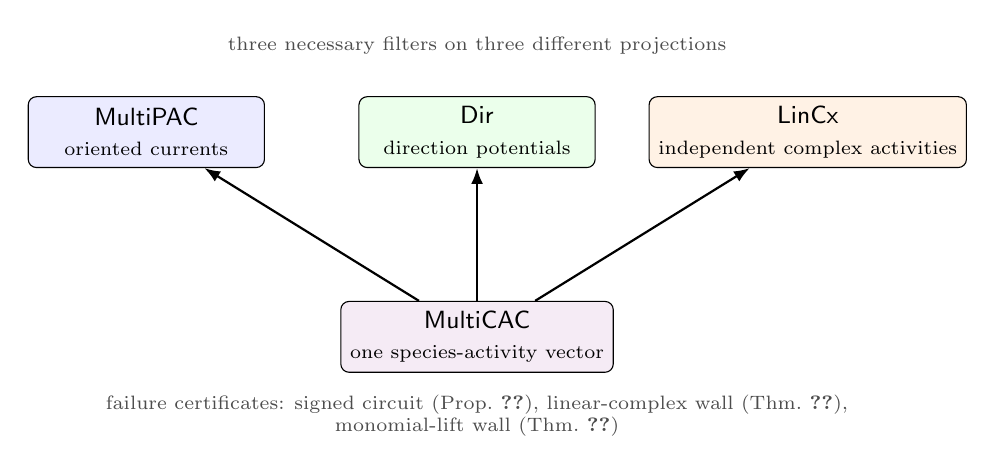
\begin{tikzpicture}[
  box/.style={draw,rounded corners=3pt,minimum width=3.0cm,minimum height=0.9cm,align=center,font=\small},
  arr/.style={-{Latex[length=2mm]},thick}]
  \node[box,fill=blue!8] (pac) at (-4.2,0) {$\MPAC$\\ \scriptsize oriented currents};
  \node[box,fill=green!8] (dir) at (0,0) {$\DIR$\\ \scriptsize direction potentials};
  \node[box,fill=orange!10] (lin) at (4.2,0) {$\LIN$\\ \scriptsize independent complex activities};
  \node[box,fill=violet!8] (cac) at (0,-2.6) {$\MCAC$\\ \scriptsize one species-activity vector};
  \draw[arr] (cac) -- (pac);
  \draw[arr] (cac) -- (dir);
  \draw[arr] (cac) -- (lin);
  \node[font=\scriptsize,text=black!70] at (0,1.1) {three necessary filters on three different projections};
  \node[font=\scriptsize,text=black!70,align=center] at (0,-3.6) {failure certificates: signed circuit (Prop.~\ref{prop:paperpair}), linear-complex wall (Thm.~\ref{thm:sch}),\\ monomial-lift wall (Thm.~\ref{thm:toric})};
\end{tikzpicture}
\caption{The four compatibility predicates. $\MCAC$ implies the three others (Lemma~\ref{lem:necessary}); the examples of this paper show that a family can satisfy any prefix of the sequence $\MPAC$, $\DIR$, $\LIN$ and fail the next requirement.}
\label{fig:layers}
\end{figure}

\subsection{Why isolated realizability does not compose}

Theorem~2 of \citep{kosc2025} states that for a single PAC and any current $v$ compatible with the directions of its reactions, there exist $\lambda>0$ and a positive concentration vector inducing $\lambda v$. The proof solves for concentrations reaction by reaction along the core, which is possible because a single PAC never has to reconcile two different currents through one reaction. Definition~\ref{def:predicates} isolates the three ways this reconciliation can fail when cores interact: the directions may be jointly unrealizable ($\DIR$ fails), the productive current magnitudes required by the different cores through the shared reactions may be inconsistent with the fixed factors ($\LIN$ fails), or the complex activities forced by the currents may fail to be monomials in a common species vector (the monomial lift fails). The remainder of the paper exhibits each failure and proves that, for the smallest interacting topology, the second failure is governed by an exact scalar window.

\section{The Strong Compatibility Hypothesis is false}\label{sec:sch}

\begin{hypothesis}[Strong Compatibility]\label{hyp:sch}
For every core family $\cF$ on every reversible network, $\MPAC\wedge\DIR\Rightarrow\MCAC$.
\end{hypothesis}

Before refuting the hypothesis we revisit the example that motivates it.

\subsection{The example of Kosc et al.\ is a direction obstruction}

Figure~4 of \citep{kosc2025} consists of two cores on the species $e_1,e_2,e_3,e_4,e_1',e_2',e_A,e_B$ and six reactions, read in the productive direction:
\begin{gather*}
 r_1:\ e_1\to e_B+e_2,\qquad r_4:\ e_A+e_4\to e_1,\qquad r_1':\ e_1'\to e_A+e_2',\qquad r_4':\ e_B+e_4\to e_1',\\
 r_2:\ e_2+e_2'\to e_3,\qquad r_3:\ e_3\to 2e_4 .
\end{gather*}
The two cores are
\[
 (\{e_1,e_2,e_3,e_4\},\{r_1,r_2,r_3,r_4\})\qquad\text{and}\qquad(\{e_1',e_2',e_3,e_4\},\{r_1',r_2,r_3,r_4'\});
\]
they share $r_2$ and $r_3$, and the external species $e_A,e_B$ are retained in the ambient network.

\begin{proposition}\label{prop:paperpair}
For every choice of positive factors, the two cores above are PACs, the family with all reactions oriented forward is $\MPAC$, and it is neither $\DIR$ nor $\MCAC$.
\end{proposition}

\begin{proof}
The current $v=(v_1,v_2,v_3,v_4,v_1',v_4')=(6,5,4,7,6,7)$ gives production residual exactly $1$ on every species of each core: for instance $e_4$ receives $2v_3-v_4=1$ from the left core and $2v_3-v_4'=1$ from the right. PAC minimality is a finite case analysis on submotifs, carried out in the formalization (Section~\ref{sec:formal}). For direction incompatibility, note that the six displacement vectors $\alpha_r-\beta_r$ sum to zero: the multiset of consumed species $\{e_1,e_A,e_4,e_1',e_B,e_4,e_2,e_2',e_3\}$ equals the multiset of produced species. Hence $w=(1,1,1,1,1,1)$ is a signed circuit and Lemma~\ref{lem:circuit} applies. Finally $\MCAC$ fails by Lemma~\ref{lem:necessary}; the formalization proves it directly by multiplying the monomial inequalities $z_{e_B}z_{e_2}<z_{e_A}z_{e_4}$, $z_{e_A}z_{e_2'}<z_{e_B}z_{e_4}$ and $z_{e_4}^2<z_{e_2}z_{e_2'}$ that positive forward currents would force.
\end{proof}

So the original incompatibility is purely topological: the six reactions form a closed stoichiometric cycle, and no chemical potential can drive every reaction of such a cycle forward. The barriers play no role. Hypothesis~\ref{hyp:sch} is precisely the statement that direction obstructions are the only ones. They are not.

\subsection{Two triangles with a shared edge}

\begin{figure}[t]
\centering
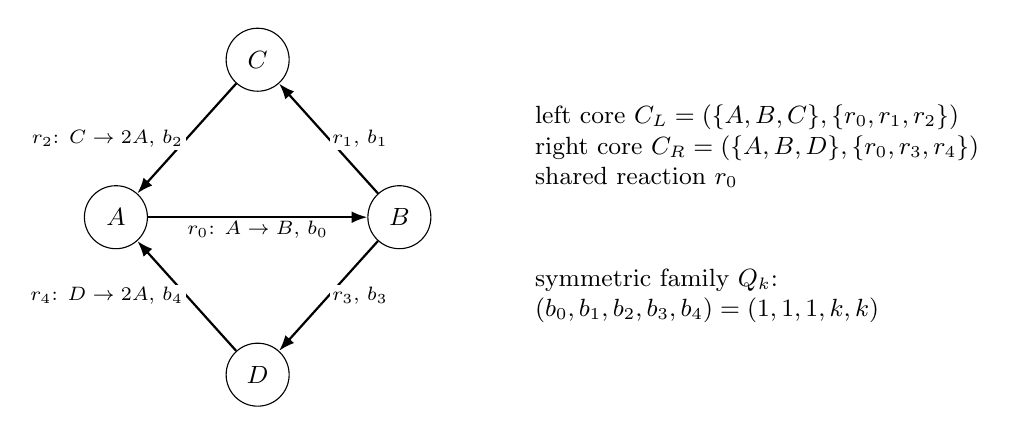
\begin{tikzpicture}[
  sp/.style={circle,draw,minimum size=8mm,font=\small,inner sep=1pt},
  rx/.style={-{Latex[length=2mm]},thick},
  lab/.style={font=\scriptsize,fill=white,inner sep=1pt}]
  \node[sp] (A) at (0,0) {$A$};
  \node[sp] (B) at (3.6,0) {$B$};
  \node[sp] (C) at (1.8,2.0) {$C$};
  \node[sp] (D) at (1.8,-2.0) {$D$};
  \draw[rx] (A) -- node[lab,below] {$r_0$: $A\to B$, $b_0$} (B);
  \draw[rx] (B) -- node[lab,right] {$r_1$, $b_1$} (C);
  \draw[rx] (C) -- node[lab,left] {$r_2$: $C\to 2A$, $b_2$} (A);
  \draw[rx] (B) -- node[lab,right] {$r_3$, $b_3$} (D);
  \draw[rx] (D) -- node[lab,left] {$r_4$: $D\to 2A$, $b_4$} (A);
  \node[font=\small,align=left,anchor=west] at (5.2,0.9) {left core $C_L=(\{A,B,C\},\{r_0,r_1,r_2\})$\\ right core $C_R=(\{A,B,D\},\{r_0,r_3,r_4\})$\\ shared reaction $r_0$};
  \node[font=\small,align=left,anchor=west] at (5.2,-1.0) {symmetric family $Q_k$:\\ $(b_0,b_1,b_2,b_3,b_4)=(1,1,1,k,k)$};
\end{tikzpicture}
\caption{The two-triangle network. Each triangle is a Type-I autocatalytic core with gain two; the cores share the reaction $A\rev B$.}
\label{fig:triangles}
\end{figure}

Let $Q$ be the network of Figure~\ref{fig:triangles} on species $A,B,C,D$ with reactions
\[
 r_0:\ A\rev B,\qquad r_1:\ B\rev C,\qquad r_2:\ C\rev 2A,\qquad r_3:\ B\rev D,\qquad r_4:\ D\rev 2A,
\]
factors $b_0,\dots,b_4>0$, and the two motifs $C_L=(\{A,B,C\},\{r_0,r_1,r_2\})$ and $C_R=(\{A,B,D\},\{r_0,r_3,r_4\})$. All reactions are oriented forward, from left to right as written.

\begin{lemma}\label{lem:trianglePAC}
$C_L$ and $C_R$ are PACs of $Q$ for every choice of factors. The family $\cF=\{C_L,C_R\}$ is $\MPAC$, witnessed by $v=(1,\tfrac45,\tfrac35,\tfrac45,\tfrac35)$, and $\DIR$, witnessed by $\mu=(\mu_A,\mu_B,\mu_C,\mu_D)=(-1,-\tfrac32,-\tfrac95,-\tfrac95)$.
\end{lemma}

\begin{proof}
For $v$ as stated, each of the six production residuals equals $\tfrac15$: in $C_L$, species $A$ receives $-v_0+2v_2$, $B$ receives $v_0-v_1$ and $C$ receives $v_1-v_2$, and symmetrically in $C_R$. The oriented affinities of $\mu$ are $\mu_A-\mu_B=\tfrac12$, $\mu_B-\mu_C=\tfrac3{10}$, $\mu_C-2\mu_A=\tfrac15$, $\mu_B-\mu_D=\tfrac3{10}$ and $\mu_D-2\mu_A=\tfrac15$, all positive. Both witnesses are independent of the factors.

For minimality of $C_L$ (the case of $C_R$ is symmetric), let $C'$ be an autocatalytic strict submotif with productive current $v$. Every reaction of $C'$ lies in $\{r_0,r_1,r_2\}$; the ambient reactions $r_3,r_4$ are absent. If $r_0\in\cR_{C'}$, side incidence puts $A,B\in\cS_{C'}$, and productivity of $A$ and $B$ within $C'$ reads $-v_0+2[r_2\in C']v_2>0$ and $v_0-[r_1\in C']v_1>0$; similarly $r_1\in C'$ forces $B,C\in\cS_{C'}$ with $[r_0\in C']v_0-v_1>0$ and $v_1-[r_2\in C']v_2>0$, and $r_2\in C'$ forces $C,A\in\cS_{C'}$ with $[r_1\in C']v_1-v_2>0$ and $-[r_0\in C']v_0+2v_2>0$. Checking the seven nonempty subsets of $\{r_0,r_1,r_2\}$ shows that each proper subset yields contradictory sign conditions (for example $\{r_0\}$ alone requires $-v_0>0$ and $v_0>0$), so $\cR_{C'}=\{r_0,r_1,r_2\}$, and side incidence then forces $\cS_{C'}=\{A,B,C\}$. Thus $C'$ is not strict.
\end{proof}

\begin{theorem}[Refutation of Strong Compatibility]\label{thm:sch}
With factors $(b_0,\dots,b_4)=(1,1,1,10,10)$, the family $\cF$ is $\MPAC$ and $\DIR$ but not $\LIN$, hence not $\MCAC$. In particular Hypothesis~\ref{hyp:sch} is false.
\end{theorem}

\begin{proof}
By Lemma~\ref{lem:trianglePAC} it remains to show that $\LIN$ fails. Suppose $y$ is a positive function on the complexes $A,B,C,D,2A$ whose linear currents $j_0=y_A-y_B$, $j_1=y_B-y_C$, $j_2=y_C-y_{2A}$, $j_3=10(y_B-y_D)$, $j_4=10(y_D-y_{2A})$ are positive and productive for both cores. Productivity of $C_L$ (species $A$, $B$, $C$ in turn) gives $2j_2>j_0$, $j_0>j_1$ and $j_1>j_2$, so
\[
 j_1+j_2 \;>\; 2j_2 \;>\; j_0 .
\]
Productivity of $C_R$ gives $2j_4>j_0$, $j_0>j_3$ and $j_3>j_4$, and the last two inequalities give
\[
 j_3+j_4 \;<\; 2j_0 .
\]
Now the private complex drops telescope: $j_1+j_2=y_B-y_{2A}$ and $j_3+j_4=10\,(y_B-y_{2A})$. Writing $x=y_B-y_{2A}$ we obtain $x>j_0$ and $10x<2j_0$, which is impossible for $j_0>0$.
\end{proof}

The proof never uses that $y$ comes from species activities, so the obstruction lives in the linear layer: the two branches leaving $B$ and returning to $2A$ must carry the same complex-activity drop $y_B-y_{2A}$, the left branch needs that drop to exceed the shared drop $j_0$, and with factor $10$ the right branch needs it to be below $j_0/5$. This is a conflict of magnitudes, and it suggests that the ratio of the private factors is the controlling parameter.

\section{The exact phase diagram}\label{sec:phase}

For $k>0$ let $Q_k$ be the network of Figure~\ref{fig:triangles} with factors $(1,1,1,k,k)$, and let $\cF_k$ be the family $\{C_L,C_R\}$ on $Q_k$ with all reactions oriented forward. By Lemma~\ref{lem:rebase} and Lemma~\ref{lem:trianglePAC}, $\cF_k$ is a core family, $\MPAC$ and $\DIR$ for every $k>0$.

\begin{theorem}[Two-triangle phase diagram]\label{thm:phase}
For every $k>0$,
\[
  \cF_k\ \text{is}\ \MCAC \quad\Longleftrightarrow\quad \tfrac12<k<2 .
\]
\end{theorem}

\begin{proof}
\emph{Necessity.} Let $z=(A,B,C,D)$ be a positive witness. The currents are
\[
 j_0=A-B,\quad j_1=B-C,\quad j_2=C-A^2,\quad j_3=k(B-D),\quad j_4=k(D-A^2),
\]
all positive. Put $j=j_0>0$ and $x=B-A^2$. As in the proof of Theorem~\ref{thm:sch}, productivity of $C_L$ gives $j<j_1+j_2<2j$, and $j_1+j_2=x$; productivity of $C_R$ gives $j<j_3+j_4<2j$, and $j_3+j_4=kx$. Hence $x\in(j,2j)$ and $kx\in(j,2j)$. If $k\le\tfrac12$ then $kx\le x/2<j$, and if $k\ge2$ then $kx\ge2x>2j$; either way a contradiction.

\emph{Sufficiency.} Assume $\tfrac12<k<2$ and put
\[
 q=\frac{3}{1+k},\qquad p=kq=\frac{3k}{1+k}.
\]
Then $1<q<2$ and $1<p<2$: indeed $q>1$ iff $k<2$, $q<2$ iff $k>\tfrac12$, $p>1$ iff $k>\tfrac12$ and $p<2$ iff $k<2$. For $1<t<2$ define
\[
 \delta(t)=\frac{(t-1)(2-t)}4,\qquad u(t)=\frac t2+\delta(t),\qquad v(t)=\frac t2-\delta(t),
\]
so that $u(t)+v(t)=t$ and $\tfrac12<v(t)<u(t)<1$; the last chain holds because $0<\delta(t)<\min\{\tfrac{t-1}2,\tfrac{2-t}2\}$. Let $(u_L,v_L)=(u(q),v(q))$ and $(u_R,v_R)=(u(p),v(p))$, and set
\[
 j=\frac{1}{4(q+1)},\qquad A=\tfrac12,\qquad B=A-j,\qquad C=B-u_Lj,\qquad D=B-\frac{u_Rj}{k}.
\]
Then $j<\tfrac18$, $B>0$, $C>\tfrac12-2j>0$, and $B-A^2=\tfrac14-j=qj$ by the choice of $j$. The currents are $j_0=j$, $j_1=u_Lj$, $j_2=(B-A^2)-u_Lj=v_Lj$, $j_3=u_Rj$ and $j_4=k(B-A^2)-u_Rj=(kq-u_R)j=v_Rj$; all are positive. Since $u_R<p=kq$ we have $D>B-qj=A^2>0$. Productivity of $C_L$ reads $(2v_L-1)j>0$, $(1-u_L)j>0$ and $(u_L-v_L)j>0$, and productivity of $C_R$ reads the same with $(u_R,v_R)$; all hold. Hence $z=(A,B,C,D)$ witnesses $\MCAC$.
\end{proof}

\begin{figure}[t]
\centering
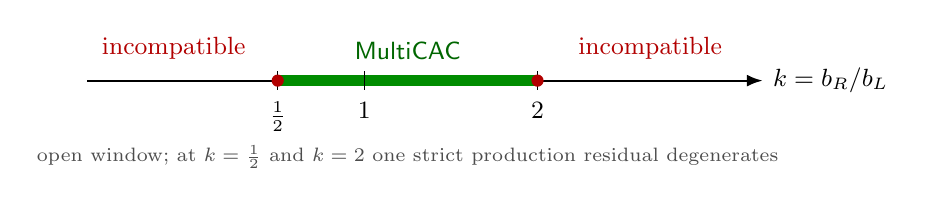
\begin{tikzpicture}[x=2.2cm]
  \draw[thick,-{Latex[length=2mm]}] (-0.6,0) -- (3.3,0) node[right,font=\small] {$k=b_R/b_L$};
  \draw[line width=4pt,green!55!black] (0.5,0) -- (2,0);
  \foreach \x/\l in {0.5/$\tfrac12$,1/$1$,2/$2$} {\draw (\x,0.12) -- (\x,-0.12); \node[below,font=\small] at (\x,-0.15) {\l};}
  \fill[red!70!black] (0.5,0) circle (2.2pt);
  \fill[red!70!black] (2,0) circle (2.2pt);
  \node[above,font=\small,green!40!black] at (1.25,0.15) {$\MCAC$};
  \node[above,font=\small,red!70!black] at (-0.1,0.15) {incompatible};
  \node[above,font=\small,red!70!black] at (2.65,0.15) {incompatible};
  \node[below,font=\scriptsize,text=black!70] at (1.25,-0.7) {open window; at $k=\tfrac12$ and $k=2$ one strict production residual degenerates};
\end{tikzpicture}
\caption{Theorem~\ref{thm:phase}. For every $k>0$ the family is $\MPAC$ and $\DIR$; a common realization exists exactly in the open window $\tfrac12<k<2$. In the symmetric transition-state family this is $|G_R^{\ddagger}-G_L^{\ddagger}|<RT\ln2$ (Section~\ref{sec:physics}).}
\label{fig:phase}
\end{figure}

\begin{remark}[Endpoints]
At $k=2$ the necessity argument gives $2x\in(j,2j)$ and $x\in(j,2j)$, whose closures meet only at $x=j$, where the residual $j_1+j_2-j_0$ of species $A$ in $C_L$ vanishes. The same happens at $k=\tfrac12$ with the roles of the cores exchanged. The window is open because productivity is strict; a weak version of productivity would close it.
\end{remark}

\begin{remark}[Scale invariance]
Only the ratio of private to shared factors enters. Replacing all five factors by $\lambda b_r$ multiplies every current by $\lambda$ and changes nothing. Replacing the shared factor $b_0$ by $\lambda b_0$ scales $j_0$ alone and is absorbed by the shared drop $A-B$; the general-factor statement below makes this explicit.
\end{remark}

\begin{proposition}[Arbitrary factors]\label{prop:generalphase}
Let $b_0,\dots,b_4>0$ be arbitrary and put $R_L=1/b_1+1/b_2$ and $R_R=1/b_3+1/b_4$. The family $\{C_L,C_R\}$ on the network of Figure~\ref{fig:triangles} is $\MCAC$ if and only if
\[
  \tfrac12<\frac{R_R}{R_L}<2 .
\]
\end{proposition}

\begin{proof}
For a positive witness $z$, write $j_0=b_0(A-B)$, $j_1=b_1(B-C)$, $j_2=b_2(C-A^2)$, $j_3=b_3(B-D)$, $j_4=b_4(D-A^2)$, and let $q=(B-A^2)/(A-B)$ be the ratio of the private complex drop to the shared drop. Then
\[
  q=\frac{j_1/b_1+j_2/b_2}{j_0/b_0}=b_0\Bigl(\frac{u_L}{b_1}+\frac{v_L}{b_2}\Bigr),\qquad u_L=\frac{j_1}{j_0},\ v_L=\frac{j_2}{j_0},
\]
and productivity of $C_L$ is exactly $\tfrac12<v_L<u_L<1$. By Theorem~\ref{thm:interface} below, the set of values of $q$ compatible with $C_L$ is the open interval $(b_0R_L/2,\,b_0R_L)$; likewise for $C_R$ it is $(b_0R_R/2,\,b_0R_R)$. Because both branches leave $B$ and return to $2A$, the ratio $q$ is literally the same quantity for both cores, so a common witness forces the two intervals to intersect, which by Corollary~\ref{cor:compose} with $m_L=m_R=2$ is the displayed condition. Conversely, given $q$ in both intervals, Theorem~\ref{thm:interface} provides $(u_L,v_L)$ and $(u_R,v_R)$ with $\tfrac12<v<u<1$ realizing $q$ on each side. Choose $A=\tfrac12$ and $B=(A^2+qA)/(1+q)\in(A^2,A)$, so that $B-A^2=q(A-B)$; put $j_0=b_0(A-B)$, $C=B-u_Lj_0/b_1$ and $D=B-u_Rj_0/b_3$. Then $C-A^2=(B-A^2)-u_Lj_0/b_1=v_Lj_0/b_2>0$ by the defining identity of $q$, so $C>A^2>0$, and the currents through $C_L$ are $j_0$, $u_Lj_0$, $v_Lj_0$; the same holds on the right. Productivity follows as in Theorem~\ref{thm:phase}.
\end{proof}

The symmetric family has $R_L=2$ and $R_R=2/k$, so Proposition~\ref{prop:generalphase} recovers Theorem~\ref{thm:phase}. The proposition is proved here by hand on top of the formally verified interval theorem; the formalization covers the literal symmetric family (Section~\ref{sec:notformal}).

\section{The interface calculus}\label{sec:interface}

The proofs of Section~\ref{sec:phase} used one scalar per core: the ratio of the complex-activity drop across the private branch to the drop across the shared reaction. This section shows that the scalar carries all the information of a triangular core, for arbitrary gain and factors, and that two eliminated cores compose by intersecting intervals.

\begin{figure}[t]
\centering
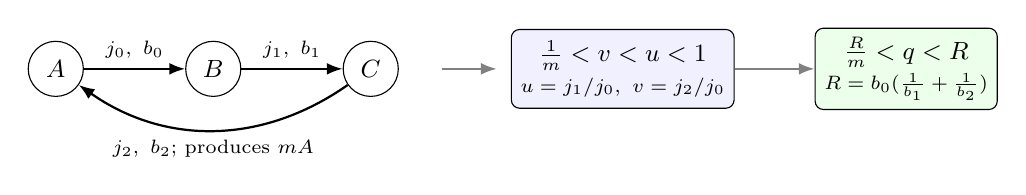
\begin{tikzpicture}[
  sp/.style={circle,draw,minimum size=7mm,font=\small,inner sep=1pt},
  rx/.style={-{Latex[length=2mm]},thick},
  box/.style={draw,rounded corners=3pt,minimum height=1.0cm,align=center,font=\small},
  lab/.style={font=\scriptsize}]
  \node[sp] (A) at (0,0) {$A$};
  \node[sp] (B) at (2,0) {$B$};
  \node[sp] (C) at (4,0) {$C$};
  \draw[rx] (A) -- node[lab,above] {$j_0,\ b_0$} (B);
  \draw[rx] (B) -- node[lab,above] {$j_1,\ b_1$} (C);
  \draw[rx] (C) to[bend left=35] node[lab,below] {$j_2,\ b_2$; produces $mA$} (A);
  \node[box,fill=blue!6] (cone) at (7.2,0) {$\tfrac1m<v<u<1$\\ \scriptsize $u=j_1/j_0,\ v=j_2/j_0$};
  \node[box,fill=green!8] (int) at (10.8,0) {$\tfrac Rm<q<R$\\ \scriptsize $R=b_0(\tfrac1{b_1}+\tfrac1{b_2})$};
  \draw[rx,gray] (4.9,0) -- (5.6,0);
  \draw[rx,gray] (cone) -- (int);
\end{tikzpicture}
\caption{Theorem~\ref{thm:interface}. Literal productive currents of a gain-$m$ triangle, the normalized productive cone, and the exact interval of the interface response $q$.}
\label{fig:interface}
\end{figure}

\begin{definition}[Literal triangle currents]\label{def:literal}
Let $m>1$ and $b_0,b_1,b_2>0$. Real numbers $(j_0,j_1,j_2)$ are \emph{literal productive currents} of the triangle $A\to B\to C\to mA$ with these factors if
\begin{equation}\label{eq:productive}
  j_0>0,\qquad mj_2-j_0>0,\qquad j_1-j_2>0,\qquad j_0-j_1>0 ,
\end{equation}
that is, if $j_0$ is forward and the net production of $A$, $C$ and $B$ is strictly positive. The \emph{interface response} of such currents is
\begin{equation}\label{eq:response}
  q=b_0\Bigl(\frac{j_1}{b_1j_0}+\frac{j_2}{b_2j_0}\Bigr).
\end{equation}
\end{definition}

When the currents come from species activities, $j_1/b_1+j_2/b_2=(B-C)+(C-A^m)=B-A^m$ and $j_0/b_0=A-B$, so $q$ is the ratio of the private drop $B-A^m$ to the shared drop $A-B$ in complex-activity space. Definition~\ref{def:literal} does not assume this; it works with currents alone. The gain $m$ is allowed to be any real number greater than one, although only integers arise from stoichiometry.

\begin{theorem}[Literal interface projection]\label{thm:interface}
Let $m>1$ and $b_0,b_1,b_2>0$, and put $R=b_0(1/b_1+1/b_2)$. A real number $q$ is the interface response of some literal productive currents if and only if
\[
  \frac Rm<q<R .
\]
\end{theorem}

\begin{proof}
Normalize by $j_0>0$: with $u=j_1/j_0$ and $v=j_2/j_0$, the conditions~\eqref{eq:productive} become $\tfrac1m<v<u<1$, and~\eqref{eq:response} becomes $q=xu+yv$ with $x=b_0/b_1$ and $y=b_0/b_2$; conversely any $(u,v)$ in this cone gives literal currents $(1,u,v)$. So it suffices to show that the image of the open cone $\{\tfrac1m<v<u<1\}$ under $(u,v)\mapsto xu+yv$ is exactly the interval $((x+y)/m,\,x+y)$.

If $\tfrac1m<v<u<1$ then $xu+yv>x/m+y/m$ and $xu+yv<x+y$ because $x,y>0$. Conversely let $(x+y)/m<q<x+y$ and put $S=x+y$, $t=q/S$, $\ell=1/m$ and
\[
  e=\frac{(t-\ell)(1-t)}{2S},\qquad u=t+ey,\qquad v=t-ex .
\]
Then $\ell<t<1$, $e>0$, and $xu+yv=St=q$. Moreover $ex<t-\ell$ because $(1-t)x<x<2S$, and $ey<1-t$ because $(t-\ell)y<y<2S$; hence $\ell<v$ and $u<1$, while $u-v=e(x+y)>0$. Thus $(u,v)$ lies in the cone and realizes $q$.
\end{proof}

\begin{corollary}[Composition of two interfaces]\label{cor:compose}
Let $m_L,m_R>1$ and $R_L,R_R>0$. The intervals $(R_L/m_L,R_L)$ and $(R_R/m_R,R_R)$ intersect if and only if
\[
  \frac1{m_L}<\frac{R_R}{R_L}<m_R .
\]
\end{corollary}

\begin{proof}
Two nonempty open intervals $(a,b)$ and $(c,d)$ intersect if and only if $a<d$ and $c<b$. Here $a<d$ reads $R_L/m_L<R_R$ and $c<b$ reads $R_R/m_R<R_L$.
\end{proof}

Corollary~\ref{cor:compose} is symmetric under exchanging the cores, as it must be: $1/m_L<R_R/R_L<m_R$ is equivalent to $1/m_R<R_L/R_R<m_L$. For the two triangles of Section~\ref{sec:phase}, $m_L=m_R=2$, $R_L=1+1=2$ and $R_R=2/k$, and the corollary gives $\tfrac12<1/k<2$, that is $\tfrac12<k<2$.

\begin{remark}[Reading the interval]\label{rem:interval}
The interval $(R/m,R)$ has a simple meaning. The two private reactions carry the entire private drop $B-A^m$; the fastest way to spend it is to put all of it on the cheaper reaction, and the productive cone forbids either reaction from carrying less than a $1/m$ share of the shared current or more than the full share. The coefficient $R$ is the sum of reciprocal private factors, a ``resistance'' of the branch, weighted by the shared factor $b_0$. A branch with large private factors (low activation energies) has small $R$ and can only carry a small drop relative to the shared one; a branch with small factors needs a large drop. Two branches sharing the same drop must therefore have resistances within the factor $m$ of each other, and for gain two within a factor of two.
\end{remark}

\begin{remark}[When the scalar is not enough]\label{rem:notenough}
The composition rule intersects two intervals of one variable $q$. This is the exact source-level condition whenever the two private branches have the same product complex, because then the private drops coincide. If the branches have different gains, the private drops $B-A^{m_L}$ and $B-A^{m_R}$ are different quantities related through the common activity of $A$, and at the species level $q_L\ne q_R$ in general. At the linear-complex level, however, $y_{m_LA}$ and $y_{m_RA}$ are independent unknowns and the two responses decouple. The next section exploits exactly this gap.
\end{remark}

\section{A monomial-lift obstruction}\label{sec:toric}

Theorem~\ref{thm:sch} showed that $\LIN$ can fail while $\MPAC$ and $\DIR$ hold. This section shows that $\LIN$ itself is not sufficient: the requirement that complex activities be monomials of one species vector can be the only thing that fails.

\subsection{Two cores on two species}

Let $Q^{\mathrm{tor}}$ be the network on species $A,B$ with the three distinct reactions
\[
 r_0:\ A\rev B\ (b_0=1),\qquad r_1:\ B\rev 2A\ (b_1=1),\qquad r_2:\ B\rev 3A\ (b_2=2),
\]
all oriented forward, and let $C_1=(\{A,B\},\{r_0,r_1\})$ and $C_2=(\{A,B\},\{r_0,r_2\})$. The two cores share $r_0$ and differ in the gain of their return reaction. No parallel or duplicate reaction channels are used; $r_1$ and $r_2$ have different product complexes.

\begin{figure}[t]
\centering
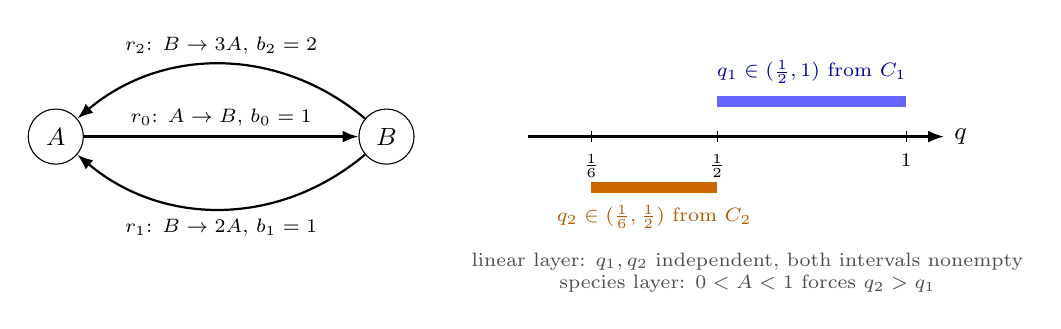
\begin{tikzpicture}[
  sp/.style={circle,draw,minimum size=7mm,font=\small,inner sep=1pt},
  rx/.style={-{Latex[length=2mm]},thick},
  lab/.style={font=\scriptsize}]
  \node[sp] (A) at (0,0) {$A$};
  \node[sp] (B) at (4.2,0) {$B$};
  \draw[rx] (A) -- node[lab,above] {$r_0$: $A\to B$, $b_0=1$} (B);
  \draw[rx] (B) to[bend left=40] node[lab,below] {$r_1$: $B\to 2A$, $b_1=1$} (A);
  \draw[rx] (B) to[bend right=40] node[lab,above] {$r_2$: $B\to 3A$, $b_2=2$} (A);
  \begin{scope}[xshift=6.0cm,x=4.8cm]
    \draw[thick,-{Latex[length=2mm]}] (0,0) -- (1.1,0) node[right,font=\small] {$q$};
    \foreach \x/\l in {0.1667/$\tfrac16$,0.5/$\tfrac12$,1/$1$} {\draw (\x,0.07) -- (\x,-0.07); \node[font=\scriptsize,anchor=north] at (\x,-0.1) {\l};}
    \draw[line width=4pt,blue!60] (0.5,0.45) -- (1,0.45);
    \node[font=\scriptsize,blue!60!black,anchor=south] at (0.75,0.55) {$q_1\in(\tfrac12,1)$ from $C_1$};
    \draw[line width=4pt,orange!80!black] (0.1667,-0.65) -- (0.5,-0.65);
    \node[font=\scriptsize,orange!70!black,anchor=north] at (0.333,-0.75) {$q_2\in(\tfrac16,\tfrac12)$ from $C_2$};
    \node[font=\scriptsize,text=black!70,align=center,anchor=north] at (0.58,-1.35) {linear layer: $q_1,q_2$ independent, both intervals nonempty\\ species layer: $0<A<1$ forces $q_2>q_1$};
  \end{scope}
\end{tikzpicture}
\caption{The monomial-lift obstruction of Theorem~\ref{thm:toric}. Each core admits a nonempty interval of interface responses, and independent complex activities can place $q_1$ and $q_2$ in their intervals simultaneously. A common species vector forces $A<1$, hence $B-A^3>B-A^2$ and $q_2>q_1$, which is incompatible with $q_1>\tfrac12>q_2$.}
\label{fig:toric}
\end{figure}

\begin{theorem}[Monomial-lift obstruction]\label{thm:toric}
$C_1$ and $C_2$ are PACs of $Q^{\mathrm{tor}}$. The family $\{C_1,C_2\}$ is $\MPAC$, $\DIR$ and $\LIN$, but not $\MCAC$.
\end{theorem}

\begin{proof}
\emph{PAC minimality.} Consider $C_1$; the argument for $C_2$ is identical with $r_2$ in place of $r_1$. Let $C'$ be an autocatalytic strict submotif with productive current $v$, so $\cR_{C'}\subseteq\{r_0,r_1\}$ is nonempty. Side incidence gives $\cS_{C'}=\{A,B\}$ whenever $\cR_{C'}\neq\emptyset$, because each of $r_0,r_1$ has $A$ on one side and $B$ on the other. If $\cR_{C'}=\{r_0\}$, productivity of $A$ and $B$ reads $-v_0>0$ and $v_0>0$; if $\cR_{C'}=\{r_1\}$ it reads $2v_1>0$ and $-v_1>0$. Both are contradictory, so $\cR_{C'}=\{r_0,r_1\}$ and $C'$ is not strict. Note that both balances are needed: the $A$-balance alone does not exclude $\{r_1\}$, since a productive current for a PAC may be negative on some reactions.

\emph{$\MPAC$.} The current $v=(1,\tfrac34,\tfrac12)$ is positive; in $C_1$ species $A$ receives $-1+2\cdot\tfrac34=\tfrac12$ and $B$ receives $1-\tfrac34=\tfrac14$; in $C_2$, $A$ receives $-1+3\cdot\tfrac12=\tfrac12$ and $B$ receives $1-\tfrac12=\tfrac12$.

\emph{$\DIR$.} With $\mu=(\mu_A,\mu_B)=(-1,-\tfrac32)$ the oriented affinities are $\mu_A-\mu_B=\tfrac12$, $\mu_B-2\mu_A=\tfrac12$ and $\mu_B-3\mu_A=\tfrac32$.

\emph{$\LIN$.} Assign $y_A=4$, $y_B=3$, $y_{2A}=\tfrac94$, $y_{3A}=\tfrac{11}4$. The linear currents are $j_0=4-3=1$, $j_1=3-\tfrac94=\tfrac34$ and $j_2=2\,(3-\tfrac{11}4)=\tfrac12$, which is the $\MPAC$ witness above; so they are positive and productive for both cores.

\emph{Not $\MCAC$.} Let $z=(A,B)$ be positive with positive productive currents $j_0=A-B$, $j_1=B-A^2$, $j_2=2(B-A^3)$. Productivity of $A$ in $C_1$ gives $2(B-A^2)>A-B$; productivity of $B$ in $C_2$ gives $A-B>2(B-A^3)$. Positivity of $j_0$ and $j_1$ gives $A^2<B<A$, hence $0<A<1$ and therefore $A^3<A^2$, so $B-A^3>B-A^2$. Combining,
\[
  A-B\;>\;2(B-A^3)\;>\;2(B-A^2)\;>\;A-B,
\]
a contradiction.
\end{proof}

In the language of Section~\ref{sec:interface}, each core here is a two-reaction core with a single private reaction, and its interface response $q=b_0j_{\mathrm{priv}}/(b_{\mathrm{priv}}j_0)$ ranges over $(b_0/(mb_{\mathrm{priv}}),\,b_0/b_{\mathrm{priv}})$; so $q_1\in(\tfrac12,1)$ and $q_2\in(\tfrac16,\tfrac12)$. The linear witness realizes $q_1=\tfrac34$ and $q_2=\tfrac14$. Under the monomial lift, $q_1=(B-A^2)/(A-B)$ and $q_2=(B-A^3)/(A-B)$ are coupled by $q_2>q_1$ whenever $A<1$, and $A<1$ is forced by the directions of $r_0$ and $r_1$. The obstruction is that the linear witness has $y_{3A}>y_{2A}$, which no species vector with $A<1$ can reproduce (Figure~\ref{fig:toric}).

\subsection{How the example was found}

The example is the smallest member of a family isolated by a theory-conditioned search rather than by a blind one. For two cores $\{A\rev B,\ B\rev mA\}$ and $\{A\rev B,\ B\rev nA\}$ with $2\le m<n$, shared factor $1$ and private factors $b_m,b_n$, the argument in the proof of Theorem~\ref{thm:toric} shows that a common species witness has $0<A<1$, hence $q_n>q_m$, while the productive cones require $q_m>1/(mb_m)$ and $q_n<1/b_n$. Therefore
\begin{equation}\label{eq:dominance}
  \frac{1}{m\,b_m}\;\ge\;\frac1{b_n}
\end{equation}
is a sufficient condition for the family to fail $\MCAC$, while both cores individually, and the linear relaxation, are unconstrained by~\eqref{eq:dominance}. Enumerating $2\le m<n\le8$ and integer $b_m,b_n\in\{1,\dots,12\}$ with exact rational arithmetic produced $441$ pairs satisfying~\eqref{eq:dominance}; ordered by $b_m+b_n$, then $b_n$, then $(m,n)$, the first is $(m,n,b_m,b_n)=(2,3,1,2)$, which is the network above. The enumeration is a discovery device: only the instance $(2,3,1,2)$ is formally verified, and we make no claim of global minimality beyond source-minimality of the two PACs and minimality within the enumerated dominance family.

\section{Formal verification}\label{sec:formal}

All theorems marked as formal in this section have been compiled in Lean~4 \citep{demoura2021}, toolchain \lean{leanprover/lean4:v4.30.0}, against the Mathlib library \citep{mathlib2020} at the matching tagged release, with a frozen \lean{lake-manifest}. Verification treats every warning as an error, rejects \lean{sorry}, extracts the requested declaration signatures, reports the axioms used, and records SHA-256 hashes of the source file, the compiled module and the declaration interface. Every verified declaration depends only on the standard axioms \lean{propext}, \lean{Classical.choice} and \lean{Quot.sound}.

\subsection{Architecture}

The development lives in the namespace \lean{ThermoCoreCompatibility}, about $2{,}600$ lines in nine files.
\begin{itemize}
\item \lean{Reaction.lean} defines \lean{ReversibleCRN} (Definition~\ref{def:crn}), complexes, complex activities and currents.
\item \lean{Source.lean} defines motifs, side incidence, productivity, strict submotifs and \lean{IsPAC} (Definition~\ref{def:motif}), and proves \lean{Motif.rebase\_isPAC} (Lemma~\ref{lem:rebase}).
\item \lean{CoreFamily.lean} defines \lean{CoreFamily}, \lean{MultiPAC} and \lean{MultiCAC} (Definitions~\ref{def:family} and~\ref{def:predicates}).
\item \lean{Direction.lean} defines \lean{DirectionCompatible}, \lean{SignedCircuit} and proves the forward half of Lemma~\ref{lem:circuit}.
\item \lean{Toric.lean} defines \lean{LinearComplexCompatible}, the toric realizability predicate on complex activities, and proves \lean{multiCAC\_iff\_positivePolyhedralToricPoint} and \lean{multiCAC\_implies\_linearComplexCompatible}.
\item \lean{InterfaceProfile.lean} contains the scalar calculus of Section~\ref{sec:interface}, from the literal current predicate \lean{LiteralTriangleCurrents} to \lean{commonResponse\_iff\_ratio}.
\item The four files \lean{PaperIncompatiblePair.lean}, \lean{MagnitudeObstructionPair.lean}, \lean{TrianglePhaseDiagram.lean} and \lean{ToricObstructionPair.lean} in the \lean{Examples} directory contain the four literal networks with their PAC proofs and witnesses.
\item \lean{Main.lean} re-exports the publication-facing statements.
\end{itemize}

The parameterized phase diagram is stated for the literal family \lean{familyAt k hk}, whose cores are PACs by \lean{rebase\_isPAC}:
\begin{lstlisting}
theorem familyAt_complete_phaseDiagram (k : ℝ) (hk : 0 < k) :
    (familyAt k hk).MultiPAC ∧
      (familyAt k hk).DirectionCompatible ∧
      ((familyAt k hk).MultiCAC ↔ 1 / 2 < k ∧ k < 2)
\end{lstlisting}
Sufficiency is organized around a certificate structure \lean{PairData} holding the nine scalars $A,B,C,D,j,u_L,v_L,u_R,v_R$ and the fourteen inequalities and identities of the proof of Theorem~\ref{thm:phase}; a separate theorem replays the certificate against the literal network. This separation of scalar construction from network replay was decisive: a monolithic proof repeatedly exhausted the elaborator's resources, and factoring the certificate made both halves routine.

The interface theorem is stated at the level of literal currents and then projected:
\begin{lstlisting}
theorem literalTriangle_interfaceProjection {m b₀ b₁ b₂ q : ℝ}
    (hm : 1 < m) (hb₀ : 0 < b₀) (hb₁ : 0 < b₁) (hb₂ : 0 < b₂) :
    InterfaceProfile.LiteralBarrierTriangleResponse m b₀ b₁ b₂ q ↔
      b₀ * (1 / b₁ + 1 / b₂) / m < q ∧ q < b₀ * (1 / b₁ + 1 / b₂)
\end{lstlisting}
and the monomial-lift obstruction is an existential over core families on the literal two-species network:
\begin{lstlisting}
theorem exists_sourceValid_genuineToricIncompatible_pair :
    ∃ F : CoreFamily (Core := ToricPair.Core) ToricPair.network,
      F.MultiPAC ∧ F.DirectionCompatible ∧
        F.LinearComplexCompatible ∧ ¬ F.MultiCAC
\end{lstlisting}
The refutation of Hypothesis~\ref{hyp:sch} is stated as the negation of the universal implication on the fixed five-reaction network, \lean{strongCompatibility\_refuted}.

\subsection{Concordance}

Table~\ref{tab:lean} lists the principal declaration behind each statement of the paper.

\begin{table}[t]
\centering
\small
\begin{tabular}{@{}>{\raggedright\arraybackslash}p{0.30\linewidth}>{\raggedright\arraybackslash}p{0.66\linewidth}@{}}
\toprule
Statement & Lean declaration (namespace \lean{ThermoCoreCompatibility}) \\
\midrule
Definitions~\ref{def:crn}--\ref{def:predicates} & \lean{ReversibleCRN}, \lean{Motif.IsPAC}, \lean{CoreFamily}, \lean{CoreFamily.MultiPAC}, \lean{CoreFamily.MultiCAC}, \lean{CoreFamily.\allowbreak DirectionCompatible}, \lean{CoreFamily.\allowbreak LinearComplexCompatible} \\
Lemma~\ref{lem:rebase} & \lean{Motif.rebase\_isPAC} \\
Lemma~\ref{lem:necessary} ($\LIN$ part) & \lean{CoreFamily.multiCAC\_\allowbreak implies\_\allowbreak linearComplexCompatible} \\
Lemma~\ref{lem:circuit} (forward) & \lean{CoreFamily.signedCircuit\_\allowbreak not\_\allowbreak directionCompatible} \\
Prop.~\ref{prop:paperpair} (PAC, $\MPAC$, $\neg\MCAC$, all factors) & \lean{PaperPair.left\_isPAC}, \lean{PaperPair.right\_isPAC}, \lean{PaperPair.paperPair\_\allowbreak multiPAC\_\allowbreak not\_\allowbreak multiCAC} \\
Lemma~\ref{lem:trianglePAC} & \lean{MagnitudePair.left\_isPAC}, \lean{MagnitudePair.right\_isPAC}, \lean{MagnitudePair.family\_multiPAC}, \lean{MagnitudePair.family\_\allowbreak directionCompatible}, \lean{TrianglePhaseDiagram.left\_isPACAt}, \lean{TrianglePhaseDiagram.right\_isPACAt} \\
Theorem~\ref{thm:sch} & \lean{MagnitudePair.magnitudeObstruction\_\allowbreak is\_\allowbreak nonToric}, \lean{sourceValid\_\allowbreak nonToric\_\allowbreak magnitudeObstruction}, \lean{strongCompatibility\_refuted} \\
Theorem~\ref{thm:phase} & \lean{TrianglePhaseDiagram.familyAt\_\allowbreak complete\_\allowbreak phaseDiagram}, \lean{triangleFamily\_\allowbreak complete\_\allowbreak phaseDiagram}; the two directions are \lean{pairMultiCAC\_\allowbreak onlyIf\_\allowbreak window} and \lean{window\_\allowbreak implies\_\allowbreak pairMultiCAC} \\
Theorem~\ref{thm:interface} & \lean{InterfaceProfile.\allowbreak weightedTriangleResponse\_iff}, \lean{InterfaceProfile.\allowbreak literalBarrierTriangleResponse\_\allowbreak iff\_\allowbreak interval}, \lean{literalTriangle\_\allowbreak interfaceProjection} \\
Corollary~\ref{cor:compose} & \lean{InterfaceProfile.\allowbreak commonResponse\_iff\_ratio} \\
Theorem~\ref{thm:toric} & \lean{ToricPair.left\_isPAC}, \lean{ToricPair.right\_isPAC}, \lean{ToricPair.\allowbreak genuineToricObstruction}, \lean{exists\_\allowbreak sourceValid\_\allowbreak genuineToricIncompatible\_\allowbreak pair} \\
\bottomrule
\end{tabular}
\caption{Correspondence between the statements of this paper and the formal declarations.}
\label{tab:lean}
\end{table}

\subsection{Receipts}

Two publication-facing declarations were replayed from a clean temporary build and matched, field by field, against their recorded receipts: toolchain, source hash, compiled-artifact hash, declaration-interface hash, declaration name and empty warning streams. The recorded SHA-256 values are listed in Table~\ref{tab:receipts}. A tooling limit is worth recording: a probe that requested the combined biconditional of the phase diagram exhausted memory after the module had compiled successfully; the two directions were therefore authenticated separately and then combined in a further verified declaration, so that no tooling limit sits inside the mathematical trust chain.

\begin{table}[t]
\centering
\scriptsize
\begin{tabular}{@{}ll@{}}
\toprule
\multicolumn{2}{@{}l@{}}{\lean{TrianglePhaseDiagram.familyAt\_complete\_phaseDiagram}} \\
\quad source & \lean{b869aee0ae4a581740858f1373d15f9106dc14d6d6c03061488f80a05a657157} \\
\quad artifact & \lean{bebbc2516686f3e848541b1e4d9f5845a72d83ae62243023fa010deccf177a7d} \\
\quad interface & \lean{b1b251239910c19142c78c07e6362bb7efe6a44a918822be9cf6adbe6d397ef3} \\
\midrule
\multicolumn{2}{@{}l@{}}{\lean{InterfaceProfile.literalBarrierTriangleResponse\_iff\_interval}} \\
\quad source & \lean{5a09b1b55927180f32d7d71c69a566f795e119e44dc35b17f476a6dfec8f01d1} \\
\quad artifact & \lean{3a4f42b260a2caf157d97f860970f6e15f44f69841b96b4c1aaf3cc36f6a2e06} \\
\quad interface & \lean{4ef11e06c3b96cbf603513e9f3fb9e3141c283602018c5436b9a4c205fdd0336} \\
\midrule
\multicolumn{2}{@{}l@{}}{\lean{ToricPair.genuineToricObstruction}} \\
\quad source & \lean{1a8c26228b2b42cce64a6d3d01fcada6640b2ac3eb013a4bc08bbf79b70e2fb8} \\
\quad artifact & \lean{c1b3288060bc5a3f0d3eed696b5a09f58ecf4fd738d9f9ad78c5030b10838337} \\
\quad interface & \lean{468fbda95f70e6c224c5c88bec56252136ce12e7a6717cd1204969bc960bde18} \\
\midrule
\multicolumn{2}{@{}l@{}}{\lean{Main.lean} (aggregate, publication-facing aliases)} \\
\quad source & \lean{3a07050e80be02e8d63b3c5884c762a4b2740b630d9a9a8f8544cc545b0f1397} \\
\quad interface & \lean{624fda48df9581c603b0bce7df545fb85a9646314e1e68078c2fccddb5305a7d} \\
\bottomrule
\end{tabular}
\caption{SHA-256 receipts of the strict verification runs.}
\label{tab:receipts}
\end{table}

\subsection{What is proved by hand}\label{sec:notformal}

The following statements are proved in this paper but are not part of the formal development, so that the reader can see precisely what has been machine-checked.
\begin{enumerate}
\item The $\MPAC$ and $\DIR$ halves of Lemma~\ref{lem:necessary}. The formal development proves the $\LIN$ half and the equivalence of $\MCAC$ with a positive polyhedral point on the monomial image; the $\DIR$ half is the one-line logarithm argument.
\item The converse half of Lemma~\ref{lem:circuit}, which is Gordan's theorem.
\item The signed circuit $w=(1,\dots,1)$ of Proposition~\ref{prop:paperpair}. The formal development proves $\neg\MCAC$ for the paper pair directly, for all factors, but does not instantiate \lean{SignedCircuit} on it.
\item Proposition~\ref{prop:generalphase}, the arbitrary-factor form of the phase diagram. Its two ingredients, the interval theorem and the composition rule, are formal; the reconstruction of species activities from a common $q$ follows the formal \lean{PairData} construction with $b_0,\dots,b_4$ in place of $(1,1,1,k,k)$ but has not itself been replayed against the literal network.
\item The general dominance inequality~\eqref{eq:dominance} and the count of $441$ enumerated pairs. Only the instance $(2,3,1,2)$ is formal; the enumeration is a bounded exact-rational script.
\item The transition-state translation of Section~\ref{sec:physics}, which is a change of variables.
\end{enumerate}
Exact rational preflight scripts were used to check the witnesses of Lemma~\ref{lem:trianglePAC}, the closed-form construction of Theorem~\ref{thm:phase} at sample values of $k$, and the interval formulas on sample factors before they were encoded; they are not part of any proof.

\section{Discussion}\label{sec:discussion}

\subsection{Physical reading}\label{sec:physics}

In transition-state theory \citep{eyring1935} the factor of reaction $r$ is $b_r=\kappa_r\,(k_{\mathrm B}T/h)\,e^{-G_r^{\ddagger}/RT}$, with a transmission coefficient $\kappa_r$ and the Gibbs activation energy $G_r^{\ddagger}$; Kosc et al.\ absorb the nonexponential prefactor and write $b_r=e^{-G_r^{\ddagger}}$ in units of $RT$. Consider the \emph{symmetric scaling family} in which both private reactions of each branch share one factor, $b_1=b_2=b_L$ and $b_3=b_4=b_R$, and both branches have equal nonexponential prefactors. Then $k=b_R/b_L=\exp[-(G_R^{\ddagger}-G_L^{\ddagger})/RT]$ and Theorem~\ref{thm:phase} reads
\[
  \cF\ \text{is}\ \MCAC \quad\Longleftrightarrow\quad \bigl|G_R^{\ddagger}-G_L^{\ddagger}\bigr|<RT\ln 2 ,
\]
about $1.7\,\mathrm{kJ\,mol^{-1}}$ at $298\,\mathrm{K}$. Two autocatalytic triangles competing for the same feeder reaction can coexist, in the static sense of this paper, only if their private activation energies are matched to within this window. Outside it, the faster branch drains the shared complex-activity drop below what the slower branch needs, regardless of the standard free energies of the species. We stress that this translation is asserted only for the symmetric family; with unequal transmission coefficients or unequal factors within a branch the exact statement is Proposition~\ref{prop:generalphase} in terms of the reciprocal-factor sums, and Remark~\ref{rem:interval} gives its meaning.

The window is not an artefact of gain two. By Corollary~\ref{cor:compose}, two triangles with gains $m_L$ and $m_R$ and equal product complexes would have the asymmetric window $1/m_L<R_R/R_L<m_R$; larger gains tolerate larger mismatches, in the direction one would expect.

\subsection{The three layers}

The examples of this paper occupy three different positions in Figure~\ref{fig:layers}. The example of Kosc et al.\ fails at the direction layer, and the failure is a signed circuit, an object that depends only on stoichiometry and orientation. The two-triangle family fails at the magnitude layer: directions are fine, but the fixed factors demand inconsistent complex-activity drops, and this is detectable by linear programming over independent complex activities. The two-species family fails only at the monomial lift: the linear program is feasible, and what fails is that the feasible complex activities must lie on the monomial image $\{(z^{c})_c:z>0\}$ of the species orthant. In the terminology of algebraic geometry this image is the positive part of a toric variety, which is why we call the last failure a toric-image obstruction; we repeat that no toric dynamical system in the sense of \citep{craciun2009} is involved.

The layers are ordered by the cost of their certificates. A signed circuit is a nonnegative kernel vector; a linear-complex wall is a Farkas certificate of an infeasible strict linear system; a monomial-lift wall is, in general, a Positivstellensatz-type certificate for the emptiness of a semialgebraic set. In the examples the last certificate is a two-line inequality, but nothing in the theory guarantees that in general.

\subsection{Limitations and open problems}

The results concern existence of a positive static witness: one activity vector for which all cores run productively at the same time. They say nothing about whether that state is a steady state of the full dynamics, whether it is stable or persistent \citep{vassena2024}, whether it is reachable, or whether it survives bounded concentrations or nonideal activities. Kosc et al.\ note that bounding concentrations can already destroy isolated realizability; the interaction of bounds with the interface calculus is untouched here.

The interface theorem covers one shared scalar and triangular private sectors. Several questions are natural.
\begin{enumerate}
\item \emph{Mixed gains at the species level.} For two triangles with different gains sharing $A\rev B$, the responses $q_L=(B-A^{m_L})/(A-B)$ and $q_R=(B-A^{m_R})/(A-B)$ are coupled through $A\in(0,1)$. Is the $\MCAC$ region in factor space still described by finitely many rational inequalities, and what replaces Corollary~\ref{cor:compose}?
\item \emph{Larger overlap graphs.} When cores overlap along a tree of shared reactions, do the intervals compose by a sequence of pairwise intersections, and when the overlap graph contains a cycle, is there a holonomy-type consistency condition around the cycle?
\item \emph{Higher-dimensional interfaces.} When two cores share more than one reaction, the interface response is a point in a polyhedron rather than an interval. The image of the productive cone under the barrier-weighted response map is then a convex set, and the monomial lift adds semialgebraic constraints. A general theory would describe exactly which such sets arise.
\item \emph{Complexity.} $\DIR$ and $\LIN$ are linear feasibility problems, so for a fixed family they are polynomial in the size of the network. $\MCAC$ asks whether a strict polynomial system has a positive solution, which is decidable but not obviously tractable. Is $\MCAC$ for a given family of PACs NP-hard, as PAC detection itself is \citep{kosc2025,andersen2012}?
\end{enumerate}

\subsection{Reproducibility}

The formal development, the exact preflight scripts, the verification driver, the replay certificate and the LaTeX source of this paper are archived together; the receipts of Table~\ref{tab:receipts} identify the verified sources bit for bit. Replaying the two publication-facing declarations requires the pinned Lean toolchain and the frozen Mathlib manifest and takes a few minutes on a workstation.

\section*{Acknowledgements}
Acknowledgements to be inserted before submission.

\bibliographystyle{unsrtnat}
\bibliography{refs}

\end{document}
